\clearpage

\begin{usecase}
  \addheading{Use-Case Description}
  \addsingletwocolumnrow{Name}{oeReplyToRequest}
  \addsingletwocolumnrow{Scope}{System}
  \addsingletwocolumnrow{Altitude}{subfunction}
  
  \addrowheading{Parameters}
  \addnumberedsinglerow{}{\msrcode{crisisID:dtCrisisID} - the crisis identification.}
  \addnumberedsinglerow{}{\msrcode{Comment:dtComment} - a comment field for the
  EMS actor to describe the situation.}
  \addnumberedsinglerow{}{\msrcode{RequestID:dtRequestID} - a unique identifier
  for a request.}
  \addnumberedsinglerow{}{\msrcode{EMSCrisisStatus:etEMSCrisisStatus} - the status of the situation(here crisis) as seen from their perspective.}
  
  \addrowheading{Primary actor(s)}
  \addnumberedsinglerow{}{\msrcode{actEMS[active]}}
  
  \addrowheading{Secondary actor(s)}
  \addnumberedsinglerow{}{\msrcode{actCoordinator[passive]}}
  
  \addrowheading{Goal(s) description}
  \addsinglerow{the \msrcode{actEMS}'s goal is to reply to a request previously sent by a coordinator.}
  
  \addrowheading{Reuse}
  \addnumberedsinglerow{}{none}

  \addrowheading{Protocol condition(s)}
  \addnumberedsinglerow{}{the \msricrash system has been deployed.}
  \addnumberedsinglerow{}{a crisis with the given ID exsits in the system.}
  \addnumberedsinglerow{}{an \msrcode{actCoordinator} has requested EMS assistance for the specified crisis.}

  \addrowheading{Pre-condition(s)}
  \addnumberedsinglerow{}{none}
  
  \addrowheading{Main post-condition(s)}
  \addnumberedsinglerow{}{the \msrcode{actEMS} has sent a reply to a received request to the system.}
  
  \addrowheading{Main success steps}
  \addalphanumberedsinglerow{}{the actor \msrcode{actEMS} sends the message \msrucname{oeReplyToRequest(dtCrisisID, dtComment, dtEMSCrisisStatus, HospitalName, ctVictim)} to the system.}
  
  \addrowheading{Step Constraints Ordering and Extensions}
  \addnumberedsinglerow{}{none}
  
  \addrowheading{Additional Information}
  \addsinglerow{This is just an example of data types that might be used in a message to reply to a request ultimately the \msrcode{actEMS} decides what he puts in to such a message.}
  
\end{usecase} 

 \clearpage

 \begin{figure}[htbp]
 \begin{center} 
 \scalebox{0.95}{
 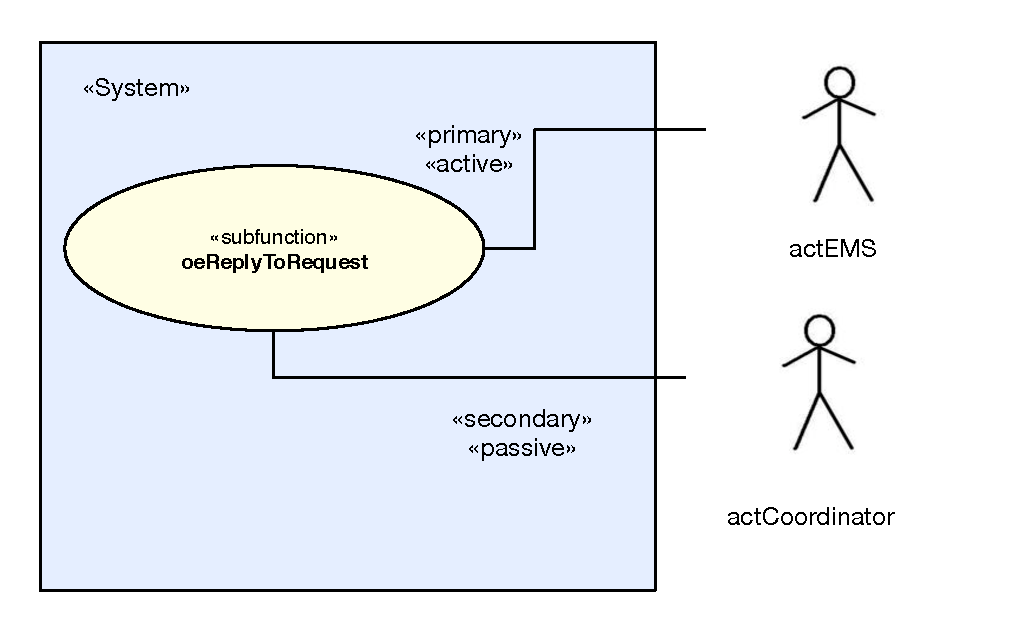
\includegraphics[width=180mm]{./images/oeReplyToRequest.eps}
 \normalsize}
 \end{center}
 \caption[\msricrash Use Case Diagram:  oeReplyToRequest Diagram]{\msricrash Use Case Diagram:  oeReplyToRequest}
 \label{fig:icrash-RE-UCD- oeReplyToRequest}
 \end{figure}
 \vspace{0.5cm}
